\section{Matched-perturbation controls}
\label{sec:controls}

Neither shift is explained by lost capability (\S\ref{sec:interp}). This section tests what determines the direction of each. If other perturbations of the same size move a model in the same direction as its 4-bit build does, the direction is a property of the model and would appear under any such perturbation. If they do not, the direction depends on the pattern of the rounding error.

\paragraph{Matched perturbations.}
For each weight matrix $W$ that the 4-bit build quantizes, embedding included, let $E = \mathrm{dequant}(Q(W)) - W$ be its rounding error. We then build fake rounding errors: dense bf16 models that perturb $W$ by the same amount as rounding does, in a different pattern. The \emph{mirror}, $W - E$, reverses the sign of the error. Three \emph{permuted} builds shuffle $E$ within each quantization group of 64, so every group keeps the same set of error values. Three \emph{Gaussian} builds replace $E$ with noise scaled to each row's norm. In every control each row is perturbed by the same norm as under rounding, and the controls lose a similar or somewhat larger amount of likelihood (Appendix~\ref{app:controls}). A \emph{dense} build, $W + E$, checks the construction. Its likelihood differs from the real quantized model's by \N{c3.qwen.gate.nlldiff} and \N{c3.llama.gate.nlldiff} nats per token, and its first token matches on \N{c3.qwen.gate.agree}\% and \N{c3.llama.gate.agree}\% of prompts. It also reproduces both shifts: \N{C3.qwenforced.dense.diff}\pp{} \N{C3.qwenforced.dense.ci} for \qwen{} and \N{C3.llamafree.dense.diff}\pp{} \N{C3.llamafree.dense.ci} for \llama, within \N{C3.qwenforced.densevsreal.absdiff} and \N{C3.llamafree.densevsreal.absdiff} points of the real builds.

We classify the direction of each shift with a decision rule. The \emph{random-control shift} is the mean shift over the permuted and Gaussian builds. A direction is the \emph{model's lean} if the random controls share the real build's sign with an interval excluding zero and the mirror does not reverse it. It is \emph{rounding-specific} if the mirror reverses it with an interval excluding zero, or if the random-control interval includes zero while the real-minus-random interval does not.

\IfMacro{C3.llamafree.summary.verdict}{Under this rule, applied to all six random draws, \qwen's shift is \N{C3.qwenforced.summary.verdict} and \llama's is \N{C3.llamafree.summary.verdict}. For \qwen, the six random controls average \N{C3.qwenforced.summary.random}\pp{} \N{C3.qwenforced.summary.random.ci}, the real build exceeds them by \N{C3.qwenforced.summary.realminusrandom}\pp{} \N{C3.qwenforced.summary.realminusrandom.ci}, and the mirror's estimate has the opposite sign (\N{C3.qwenforced.e2-mirror.diff}\pp{} \N{C3.qwenforced.e2-mirror.ci}). \llama{} shows the same pattern with the signs reversed: random controls \N{C3.llamafree.summary.random}\pp{} \N{C3.llamafree.summary.random.ci}, real minus random \N{C3.llamafree.summary.realminusrandom}\pp{} \N{C3.llamafree.summary.realminusrandom.ci}, mirror \N{C3.llamafree.e2-mirror.diff}\pp{} \N{C3.llamafree.e2-mirror.ci}. Neither mirror is significant by itself, but each differs clearly from its real build, and half of that difference is \N{C3.qwenforced.summary.odd}\pp{} \N{C3.qwenforced.summary.odd.ci} and \N{C3.llamafree.summary.odd}\pp{} \N{C3.llamafree.summary.odd.ci}. In \llama{} the two random families differ: the permuted builds shift by \N{C3.llamafree.e2-perm1.diff}, \N{C3.llamafree.e2-perm2.diff} and \N{C3.llamafree.e2-perm3.diff}\pp{} and the Gaussian builds by \N{C3.llamafree.e2-gauss.diff}, \N{C3.llamafree.e2-gauss2.diff} and \N{C3.llamafree.e2-gauss3.diff}\pp, and the part of \llama's shift that does not change sign with the error, \N{C3.llamafree.summary.even}\pp{} \N{C3.llamafree.summary.even.ci}, is up to a third of it.}{Both shifts are rounding-specific. For \qwen, the random controls average \N{C3.qwenforced.summary3.random}\pp{} \N{C3.qwenforced.summary3.random.ci}, the real build exceeds them by \N{C3.qwenforced.summary3.realminusrandom}\pp{} \N{C3.qwenforced.summary3.realminusrandom.ci}, and the mirror's estimate has the opposite sign (\N{C3.qwenforced.e2-mirror.diff}\pp{} \N{C3.qwenforced.e2-mirror.ci}). \llama{} shows the same pattern with the signs reversed: random controls \N{C3.llamafree.summary3.random}\pp{} \N{C3.llamafree.summary3.random.ci}, real minus random \N{C3.llamafree.summary3.realminusrandom}\pp{} \N{C3.llamafree.summary3.realminusrandom.ci}, mirror \N{C3.llamafree.e2-mirror.diff}\pp{} \N{C3.llamafree.e2-mirror.ci}. Neither mirror is significant by itself, but each differs clearly from its real build, and half of that difference is \N{C3.qwenforced.summary.odd}\pp{} \N{C3.qwenforced.summary.odd.ci} and \N{C3.llamafree.summary.odd}\pp{} \N{C3.llamafree.summary.odd.ci}. In \llama{} the two random families differ: the permuted builds shift by \N{C3.llamafree.e2-perm1.diff}, \N{C3.llamafree.e2-perm2.diff} and \N{C3.llamafree.e2-perm3.diff}\pp{} and the Gaussian builds by \N{C3.llamafree.e2-gauss.diff}, \N{C3.llamafree.e2-gauss2.diff} and \N{C3.llamafree.e2-gauss3.diff}\pp, and the part of \llama's shift that does not change sign with the error, \N{C3.llamafree.summary.even}\pp{} \N{C3.llamafree.summary.even.ci}, is up to a third of it.}

\begin{figure}[t]
\centering
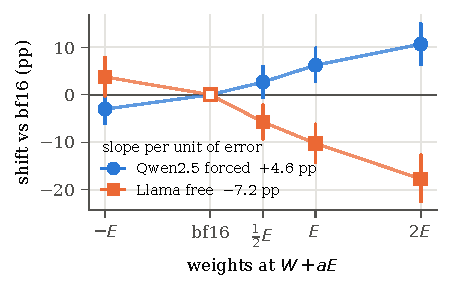
\includegraphics[width=\columnwidth]{figures/dose.pdf}
\caption{Dose. Each build is $W + aE$, where $E$ is the real 4-bit rounding error; $a=-1$ is the mirror and $a=1$ the real build. Shift against bf16 with 95\% intervals; the legend gives the slope. Every control build is in Appendix~\ref{app:controls}.}
\label{fig:dose}
\end{figure}

\paragraph{Dose.}
The mirror is the real error scaled by $-1$. Builds at $\tfrac12$ and $2$ extend it to a line through weight space, $W + aE$ (Figure~\ref{fig:dose}). In both models the shift is monotone in $a$ and near-linear over the tested range, and its estimate has the opposite sign at $a=-1$. The slopes are \N{C3.qwenforced.slope}\pp{} \N{C3.qwenforced.slope.ci} and \N{C3.llamafree.slope}\pp{} \N{C3.llamafree.slope.ci} per unit of error. The doubled builds lose much more likelihood than the real builds (\N{C3.qwenforced.e2-scale2.nllgap} and \N{C3.llamafree.e2-scale2.nllgap} nats per token, against \N{C3.qwenforced.realnllgap} and \N{C3.llamafree.realnllgap}), and the conclusion does not depend on them. The half-size build of \llama{} is more informative. Its change in likelihood (\N{C3.llamafree.e2-scale0.5.nllgap} nats per token) is probably too small for a perplexity check to detect, and it is already \N{C3.llamafree.e2-scale0.5.absdiff} points less compliant ($p=\N{C3.llamafree.e2-scale0.5.p}$).

\paragraph{Other quantizers and a second runtime.}
Other quantizers produce real rounding errors with a different structure at the same bit width. AWQ and GPTQ write the default format at \N{cap.qwen.awq.bpw} bits per weight but choose the quantized values using calibration data, and llama.cpp's Q4\_K\_M uses a different scheme in a different runtime. AWQ reproduces \qwen's shift (\N{S9.qwenforced.awq.diff}\pp{} \N{S9.qwenforced.awq.ci}, against the default build's \N{S9.qwenforced.4bit-g64.diff}) but not \llama's (\N{S9.llamafree.awq.diff}\pp{} \N{S9.llamafree.awq.ci}). Q4\_K\_M shifts neither model, and in both cells its estimate has the \emph{opposite} sign to the default build's: \N{S9.qwenforced.gguf-q4km.diff}\pp{} \N{S9.qwenforced.gguf-q4km.ci} and \N{S9.llamafree.gguf-q4km.diff}\pp{} \N{S9.llamafree.gguf-q4km.ci}. For \qwen{} its larger bit budget does not explain this, because at \N{S9.qwenforced.gguf-q4km.bpw} bits per weight it matches our \texttt{4bit-g32}, which does shift \qwen{} (\N{S6.qwen.4bit-g32.diff}\pp{}). Q4\_K\_M still changes \N{S9.qwenforced.gguf-q4km.churn}\% and \N{S9.llamafree.gguf-q4km.churn}\% of labels, without a net direction. The two runtimes do not differ significantly at bf16 (\N{S9.qwenforced.runtimebf16.diff}\pp, $p=\N{S9.qwenforced.runtimebf16.p}$; \N{S9.llamafree.runtimebf16.diff}\pp, $p=\N{S9.llamafree.runtimebf16.p}$). GPTQ contributes one cell, \llama{} at \N{S9.llamafree.gptq.diff}\pp{} \N{S9.llamafree.gptq.ci} (Holm $p=\N{S9.llamafree.gptq.pholm}$), with the same sign as the default build. The \qwen{} GPTQ build failed and is excluded, and \llama's Q8\_0 build is nominally lower but does not survive Holm correction (both in Appendix~\ref{app:prereg}). Builds at the same bit width thus differ in whether they shift a model.

\section{Refusal-direction projections}
\label{sec:direction}

The controls show that each shift depends on its rounding error, but not what that error changes inside the model. Refusal in these models is mediated by a single direction in the residual stream \citep{arditi2024refusal}, the same direction that we use to build the compliant prefixes. For every build, on the prompts of the behavioural tests, we record the projection of the model's state at the point of generation onto its bf16 refusal direction, and compare it with bf16 prompt by prompt. The analysis is correlational and identifies no circuit. We test two predictions. First, 4-bit \qwen{} under a forced start should have a \emph{lower} projection than bf16, and 4-bit \llama{} under a free start a \emph{higher} one. Second, across all builds of a cell, real and control, the change in projection should be negatively correlated with the change in compliance.

\qwen{} fits the first prediction but not the second. At the layer used for abliteration (layer \N{M1.qwenforced.layer}), the projection of its 4-bit build under a forced start is lower than bf16's (\N{M1.qwenforced.4bit-g64.mean} \N{M1.qwenforced.4bit-g64.ci}), and the mirror build's is higher (\N{M1.qwenforced.e2-mirror.mean}). The projection scales with the dose, at \N{M1.qwenforced.e2-scale0.5.mean}, \N{M1.qwenforced.4bit-g64.mean} and \N{M1.qwenforced.e2-scale2.mean} for $a = \tfrac12, 1, 2$. Across the \N{M1.qwenforced.nbuilds} builds of this cell, however, the two are not significantly correlated (Spearman $\rho=\N{M1.qwenforced.rho}$, $p=\N{M1.qwenforced.rhop}$). Several builds lower the projection nearly as much as the default build without making \qwen{} more compliant, among them a Gaussian control (\N{M1.qwenforced.e2-gauss2.mean}) and MXFP4 (\N{M1.qwenforced.mxfp4.mean}). The same 4-bit build lowers the projection further under a free start (\N{M1.qwenfree.4bit-g64.mean} \N{M1.qwenfree.4bit-g64.ci}), where its behaviour does not shift.

\llama{} fits both predictions, but weakly. The projection of its 4-bit build is slightly higher than bf16's, as predicted (\N{M1.llamafree.4bit-g64.mean} \N{M1.llamafree.4bit-g64.ci}), and the mirror's is lower (\N{M1.llamafree.e2-mirror.mean}). Across \N{M1.llamafree.nbuilds} builds the two are correlated as predicted ($\rho=\N{M1.llamafree.rho}$, $p=\N{M1.llamafree.rhop}$). However, the doubled build, which has the largest behavioural shift, changes the projection in the opposite direction (\N{M1.llamafree.e2-scale2.mean}), and under a forced start, where \llama's behaviour does not shift, the 4-bit build changes the projection by about as much (\N{M1.llamaforced.4bit-g64.mean} \N{M1.llamaforced.4bit-g64.ci}).

In both models the real error moves the state at the start of the reply along the refusal direction with the predicted sign, and the mirror moves it the other way, but this also happens in builds and settings whose behaviour does not change.
